\documentclass[journal,9pt]{IEEEtran}
%Aug 23, 2023. This template is for IEEE's Short paper/Brief article/ Techinical Correspondence, 16pt center pagewide title, 2 columns, 
%9/11pt  body text.8/9pt footnote, abstract, ref. No biographies.

% ========== Packages ==========
\usepackage[british]{babel}
\usepackage[utf8]{inputenc}
\usepackage[T1]{fontenc}
\usepackage{amsmath,amsfonts}
\usepackage{algorithmic}
\usepackage{algorithm}
\usepackage{array}

\usepackage[caption=false,font=normalsize,labelfont=sf,textfont=sf]{subfig}
%Please use all packages specified with their parameters otherwise the results may not be the same.

\usepackage{textcomp}
\usepackage{stfloats}
\usepackage{url}
\usepackage{verbatim}
\usepackage{graphicx}
\usepackage{cite}
\usepackage[hidelinks]{hyperref}
\hyphenation{op-tical net-works semi-conduc-tor IEEE-Xplore}
%updated: Aug 30, 2022: Dead links and support email addresses were removed; Running-head, article title were changed to genric publication
% updated with editorial comments 8/9/2021
\usepackage{siunitx}

% ========== Custom definitions ==========
\newcommand{\frequencyrange}{\qtyrange{4.8}{5.7}{\giga\hertz}}
\newcommand{\TEM}{\text{TEM}}
\newcommand{\TE}[2]{\text{TE}_{#1#2}}
\newcommand{\TM}[2]{\text{TM}_{#1#2}}

% ========== Document ==========
\begin{document}

% ========== Title ==========
\title{\huge{Hexagonal Waveguide Polarizer for a Compact Dual Circularly Polarized Antenna}}

% ========== Authors ==========
\author{Martin Šimák,~\IEEEmembership{Student Member,~IEEE,}~Ding-Bing Lin,~\IEEEmembership{Member,~IEEE,}~and~Pavel Hazdra,~\IEEEmembership{Member,~IEEE}%
\thanks{M. Šimák is with the Microwave Sensing, Signals and Systems (MS3) Group, Delft University of Technology, 2628 CD Delft, The Netherlands (email: m.simak@tudelft.nl).}%
\thanks{D. B. Lin is with the Department of Electronic and Computer Engineering, National Taiwan University of Science and Technology, Taipei City, Taiwan (email: db.lin@mail.ntust.edu.tw).}%
\thanks{P. Hazdra is with the Department of Electromagnetic Field, Czech Technical University in Prague, Prague, Czechia (email: hazdrap@fel.cvut.cz).}%
}

% ========== Headers ==========
\markboth{IEEE Transactions on Antennas and Propagation}%
{M. Šimák, D.-B. Lin, and P. Hazdra: Hexagonal Waveguide Polarizer for a Compact Dual Circularly Polarized Antenna}

% \IEEEpubid{0000--0000~\copyright~2023 IEEE}
% Remember, if you use this you must call \IEEEpubidadjcol in the second
% column for its text to clear the IEEEpubid mark.

\maketitle

\begin{abstract}
    This paper introduces a dual circularly polarized (CP) antenna for the 4.8~GHz to 5.7~GHz band. The antenna integrates a hexagonal waveguide polarizer, a dual-coaxial feed, and a conical horn. A high-isolation feeding structure is proposed, and a simplified version is implemented for robust manufacturability. Right-hand (RHCP) and left-hand (LHCP) circular polarization are achieved by selectively exciting fundamental modes within the square waveguide. Measurements of the fabricated prototype confirm an axial ratio below 4~dB and a gain of approximately 12~dBi to 15~dBi across the band, demonstrating excellent agreement with simulations. The proposed antenna offers a promising solution for satellite communications, radar, and related wireless applications requiring dual CP operation.
\end{abstract}

\begin{IEEEkeywords}
Circular polarization, waveguide polarizer, dual feed, conical horn antenna, hexagonal waveguide, eigenmode analysis, electromagnetic simulation.
\end{IEEEkeywords}

% ========== Section I: Introduction ==========
\section{Introduction}

\IEEEPARstart{D}{ual} circularly polarized (CP) antennas are essential components in various wireless systems, including satellite communications and radar, requiring both right-hand (RHCP) and left-hand (LHCP) polarization capabilities~\cite{jia-et-al:dual-circularly-polarized-antennas-with-low-cross-polarization-for-gnss-r-applications, zang-et-al:single-layer-dual-circularly-polarized-antenna-elements-for-automotive-radar-at-77-ghz}. Waveguide-based polarizers offer a robust solution for achieving dual-CP operation due to their inherent ability to support two orthogonal, degenerate modes. This introduction briefly reviews existing waveguide polarizer techniques and introduces a novel, easily manufacturable design approach.

Traditional waveguide polarizers for generating circular polarization typically fall into three main categories: dielectric, septum, and iris polarizers~\cite{shuliak-et-al:modern-microwave-polarizers-and-their-electromagnetic-characteristics, arora-et-al:dielectric-polarizer-based-potter-horn-antenna-for-deep-space-on-board-ttc-uplink-applications}. Dielectric polarizers, while simple to implement, suffer from narrow bandwidths and dielectric losses, limiting their power handling capabilities~\cite{melendro-jimenez-et-al:a-novel-logarithmic-spiral-shaped-3d-printed-dielectirc-polarizer-for-dual-circularly-polarized-conical-beam-radiation-patterns-in-the-ka-band}. Septum polarizers offer good power handling and dual-CP generation but can be bulky and complex to reconfigure~\cite{ruiz-cruz-et-al:compact-reconfigurable-waveguide-circular-polarizer, wang-et-al:novel-square-rectangle-waveguide-septum-polarizer}. Iris polarizers, capable of higher power operation, often face challenges with overmoding and require intricate design for wideband performance~\cite{song-et-al:design-of-wideband-quad-ridge-waveguide-polarizer, virone-et-al:optimum-iris-set-concept-for-waveguide-polarizers, piltyay-et-al:new-tunable-iris-post-square-waveguide-polarizers-for-satelliste-information-systems}. Recent work has explored alternative waveguide geometries, including elliptical and those with shaped metallic inserts, to leverage mode dispersion for polarization control~\cite{yu-et-al:a-wideband-circularly-polarized-horn-antenna-with-a-tapered-elliptical-waveguide-polarizer, rud-shpachenko:polarizers-on-sections-of-square-waveguides-with-inner-corner-ridges, bhardwaj-volakis:hexagonal-waveguides-new-class-of-waveguides-for-mmwave-circularly-polarized-horns, bhardwaj-volakis:hexagonal-waveguide-based-circularly-polarized-horn-antennas-for-submmwave-terahertz-band, bhardwaj-volakis:circularly-polarized-horn-antennas-for-terahertz-communications-using-differential-mode-dispersion-in-hexagonal-waveguides, garcia-marin-masa-campos:bowtie-shaped-radiating-element-for-single-and-dual-circular-polarization}.

This paper presents a novel dual-CP antenna operating in the $\frequencyrange$ band. The antenna system integrates a specially designed square waveguide polarizer, a dual-coaxial feed, and a conical horn. The core of the design lies in the polarizer, which achieves the required 90-degree phase shift between orthogonal modes through geometric modifications to the waveguide cross-section, inspired by approaches used in patch antennas~\cite{armin-et-al:modification-of-a-2g2hz-sband-rectangular-patch-microstrip-antenna-using-truncated-corner-method-for-satellite-applications}. This approach offers a balance between performance, compactness, and ease of fabrication. The dual-coaxial feed provides the necessary excitation for both RHCP and LHCP operation, while the conical horn provides the desired gain characteristics. The design was validated through electromagnetic simulations using CST Studio Suite~\cite{cst}, and experimental results from a fabricated prototype demonstrate excellent agreement with simulations. Key performance metrics include an axial ratio below 4 dB and a gain of approximately $\qtyrange{12}{15}{dBi}$ across the operating band.

The rest of this paper is organized as follows: Section~\ref{sec:passive-radiating-structure-design} details the design of the passive radiating components. Section~\ref{sec:dual-mode-feeding-structure-and-integration} describes the feeding structure and system integration. Section~\ref{sec:experimental-validation} presents the experimental validation of the fabricated prototype, followed by the conclusion in Section~V.


% ========== Section II: Passive Radiating Structure Design ==========
\section{Passive Radiating Structure Design}
\label{sec:passive-radiating-structure-design}

% ========== Section II-A: Hexagonal Waveguide Polarizer ==========
\subsection{Hexagonal Waveguide Polarizer}
\label{subsec:hexagonal-waveguide-polarizer}

\begin{figure}[b]
    \centering
    \includegraphics[width=.8\linewidth]{src/polarizer_perspective.png}
    \caption{\label{fig:polarizer-perspective}Exploded view of the hexagonal waveguide polarizer.}
\end{figure}

The proposed dual-CP antenna utilizes a novel square waveguide polarizer design based on introducing geometric modifications to the waveguide cross-section. This approach, inspired by techniques used in patch antennas~\cite{armin-et-al:modification-of-a-2g2hz-sband-rectangular-patch-microstrip-antenna-using-truncated-corner-method-for-satellite-applications}, involves inserting simple shapes into opposing corners of a standard square waveguide. Specifically, triangular prisms are used, forming a hexagonal-like cross-section (see Fig.~\ref{fig:polarizer-perspective}) similar to structures explored in~\cite{bhardwaj-volakis:hexagonal-waveguides-new-class-of-waveguides-for-mmwave-circularly-polarized-horns}. This geometry was chosen for its relative ease of fabrication compared to curved inserts exposed in~\cite{garcia-marin-masa-campos:bowtie-shaped-radiating-element-for-single-and-dual-circular-polarization}, while offering effective field manipulation for polarization control. A trade-off for this manufacturability is a moderately wide operating bandwidth, as the principle relies on mode dispersion induced by the resonant nature of the inserts.

\begin{figure}[!b]
    \centering
    \includegraphics[width=\linewidth]{src/polarizer_sweep.eps}
    \caption{\label{fig:polarizer-sweep}Performance of the hexagonal waveguide polarizer cross-section for different chamfering widths $w$. The figure illustrates the length required for a $\pi/2$ phase shift between the two modes ($L_\perp$), and the amplitude ratio of the two orthogonal modes ($E_2/E_1$).}
\end{figure}

The fundamental principle relies on breaking the degeneracy of the fundamental $\TE 10$ and $\TE 01$ modes of the square waveguide. The inserted prisms perturb the fields, resulting in two new orthogonal eigenmodes with distinct propagation constants, $k_1$ and $k_2$. This difference in propagation constants, $\Delta k_L$, causes a differential phase shift, $\Delta\phi_L$, to accumulate between the two modes as they propagate along the polarizer length $L$. The design objective is to achieve the differential phase shift of approximately $\pi/2$ across the desired operating band while maintaining approximately equal amplitudes for the two modes. By definition, achieving the first condition yields elliptical polarization. Furthermore, simultaneously fulfilling the latter condition results in circular polarization. Due to the diagonal symmetry of the structure, achieving optimal performance for one sense of CP (e.g., RHCP from $\TE 01$) inherently ensures similar performance for the opposite sense (LHCP from $\TE 10$).

\begin{figure}[!b]
    \centering
    \subfloat[]{\includegraphics[width=\linewidth]{src/polarizer_radiation.eps}}\\
    \subfloat[]{\includegraphics[width=\linewidth]{src/polarizer_ar.eps}}
    \caption{\label{fig:polarizer-radiation}(a) Far-field radiation patterns in the elevation plane ($\varphi=\ang{90}$) of the open-ended hexagonal waveguide polarizer at $\qty{5.2}{GHz}$. (b) Boresight axial ratio frequency response, which is identical for both ports.}
\end{figure}

Initial investigations comprised the eigenmode analysis in CST Studio Suite of square waveguides with triangular prisms for inserts and circular waveguides with cylindrical segments. Assuming uniform waveguides, the key metrics evaluated were the specific phase shift and the amplitude ratio of the modes. While both geometries showed similar mode cutoff frequency dispersion, the square waveguide configuration demonstrated superior phase dispersion characteristics while maintaining a lower amplitude dispersion gradient across the target frequency band. Consequently, the square waveguide with triangular inserts was selected for further development. The specific design targets the $\frequencyrange$ band, relevant for satellite communications and radar applications. An initial square waveguide side length of $a = \qty{50}{mm}$ was chosen, corresponding to the standard WR-187 waveguide~\cite{spinner:waveguide-specifications}, though the inserts modify the cutoff frequencies. Eigenmode simulations confirmed this dimension provides adequate bandwidth considering the lower cutoff frequency introduced by the inserts.

A parametric sweep varying the chamfering width $w$ was performed. The goal was to find a cross-section facilitating an acceptable trade-off between the polarizer length required to achieve sufficient mode dispersion at the output (i.e., to fulfil the condition on circular polarization), while maintaining close-to-equal mode amplitudes. Based on the sweep results (summarized in Fig.~\ref{fig:polarizer-sweep}), a chamfering width of $w = \qty{23}{mm}$ and a polarizer length of $L = 2.2\lambda \approx \qty{126}{mm}$ were selected.

To validate the design, a full-wave simulation of the finalized polarizer section, connected between two standard $a \times a$ square waveguide sections (input and output), was performed. The input was fed with the fundamental $\TE 10$ or $\TE 01$ mode, providing the necessary excitation to evaluate the far-field axial ratio from the radiated fields at the output waveguide aperture. The results, shown in Fig.~\ref{fig:polarizer-radiation}, confirm excellent performance, with the AR remaining below $\qty{2}{dB}$ across the entire $\frequencyrange$ band and reaching near $\qty{0}{dB}$ around the centre frequency. Representative radiation patterns further confirm the generation of high-purity CP waves and the diagonal symmetry of the polarizer structure assumed earlier.

In addition to axial ratio, the cross-polarization discrimination (XPD) was evaluated in the boresight direction for both excitation ports. The maximum XPD reaches approximately $\qty{38}{dB}$, while the overall XPD remains better than $\qty{18}{dB}$ across the operating band, directly corresponding to the observed axial ratio. Furthermore, the $\qty{2}{dB}$ axial ratio beamwidth (ARBW) is approximately $\qty{80}{\degree}$, indicating robust polarization purity over a wide angular range.


% ========== Section II-B: Conical Horn Radiator ==========
\subsection{Conical Horn Radiator}
\label{subsec:conical-horn-radiator}

A conical horn antenna was selected to radiate the wave from the polarizer into free space, chosen for its axial symmetry and suitability for CP applications. The horn was initially synthesized using Antenna Magus~\cite{antenna-magus} for a target gain of $\qty{15}{dBi}$. It was then adapted to the square aperture of the polarizer and its dimensions optimized in CST Studio Suite, guided by the well-understood relationship between gain and horn geometry~\cite{aboserwal-et-al:conical-horn-gain-and-amplitude-patterns}. The final dimensions of flare diameter $D_f = \qty{130}{mm}$ and flare length $L_f = \qty{70}{mm}$ were chosen to provide sufficient gain margin while maintaining a compact footprint. Simulation of the horn confirmed excellent polarization purity and a peak gain of $\qty{15.5}{dBi}$.


% ========== Section III: Dual-Mode Feeding Structure and Integration ==========
\section{Dual-Mode Feeding Structure and Integration}
\label{sec:dual-mode-feeding-structure-and-integration}

To facilitate the excitation of a circularly polarized wave in the subsequent antenna sections, a feeding structure capable of launching the two degenerate fundamental modes, $\TE 10$ and $\TE 01$, within a square waveguide is required. The design must ensure independent control of each mode with acceptable port-to-port isolation. Our approach begins with the well-understood principles of a single coaxial-to-waveguide transition and extends them to a novel dual-feed configuration that achieves excellent isolation and ultimately to the practical implementation chosen for fabrication.

\subsection{High-Isolation Feed Concept}

The foundation of our design is the right-angle coaxial-to-waveguide transition, a widely documented method~\cite{fabregas-et-al:coaxial-to-rectangular-waveguide-transitions}. In this configuration, the inner conductor of a coaxial cable protrudes into the waveguide, forming a monopole-like probe. The efficiency of power transfer into the desired waveguide mode is primarily governed by two parameters: the probe length, $l$, and its distance from the short-circuited end of the waveguide, the back-short, $d$. For optimal performance, the probe length is tuned to be near a quarter of the operating wavelength ($l \approx \lambda/4$), accounting for the probe's finite thickness and fringing capacitance. The distance to the back-short is set to approximately a quarter of the guide wavelength ($d \approx \lambda_g/4$) to ensure that the wave reflected by the back-short constructively interferes with the forward-propagating wave radiated by the probe. While higher-order resonances exist for $d = (2\nu+1)\lambda_g/4$ where $\nu \in \mathbb{N}$, these result in significantly narrower bandwidths and are thus avoided.

\begin{figure}[!b]
    \centering
    \includegraphics[width=.93\linewidth]{src/dual_feed_side_cut_view.png}
    \caption{\label{fig:dual-feed-conceptual}Conceptual design of the high-isolation dual-feed structure with a wire grating polarizer.}
\end{figure}

To excite the orthogonal mode, a second, perpendicularly oriented probe is introduced. A simplistic implementation, placing both probes within the same transverse plane, was initially assumed to result in high mutual coupling, prompting the search for a more sophisticated approach. While longitudinally displacing one port can improve isolation, it necessitates retuning its back-short distance, which, as previously noted, is optimal only at a specific distance, limiting performance.

\begin{figure}[!t]
    \centering
    \includegraphics[width=\linewidth]{src/dual_feed_sparameters.eps}
    \caption{\label{fig:dual-feed-sparameters}Simulated S-parameters of the conceptual high-isolation dual-feed structure.}
\end{figure}

\begin{figure}[!b]
\centering
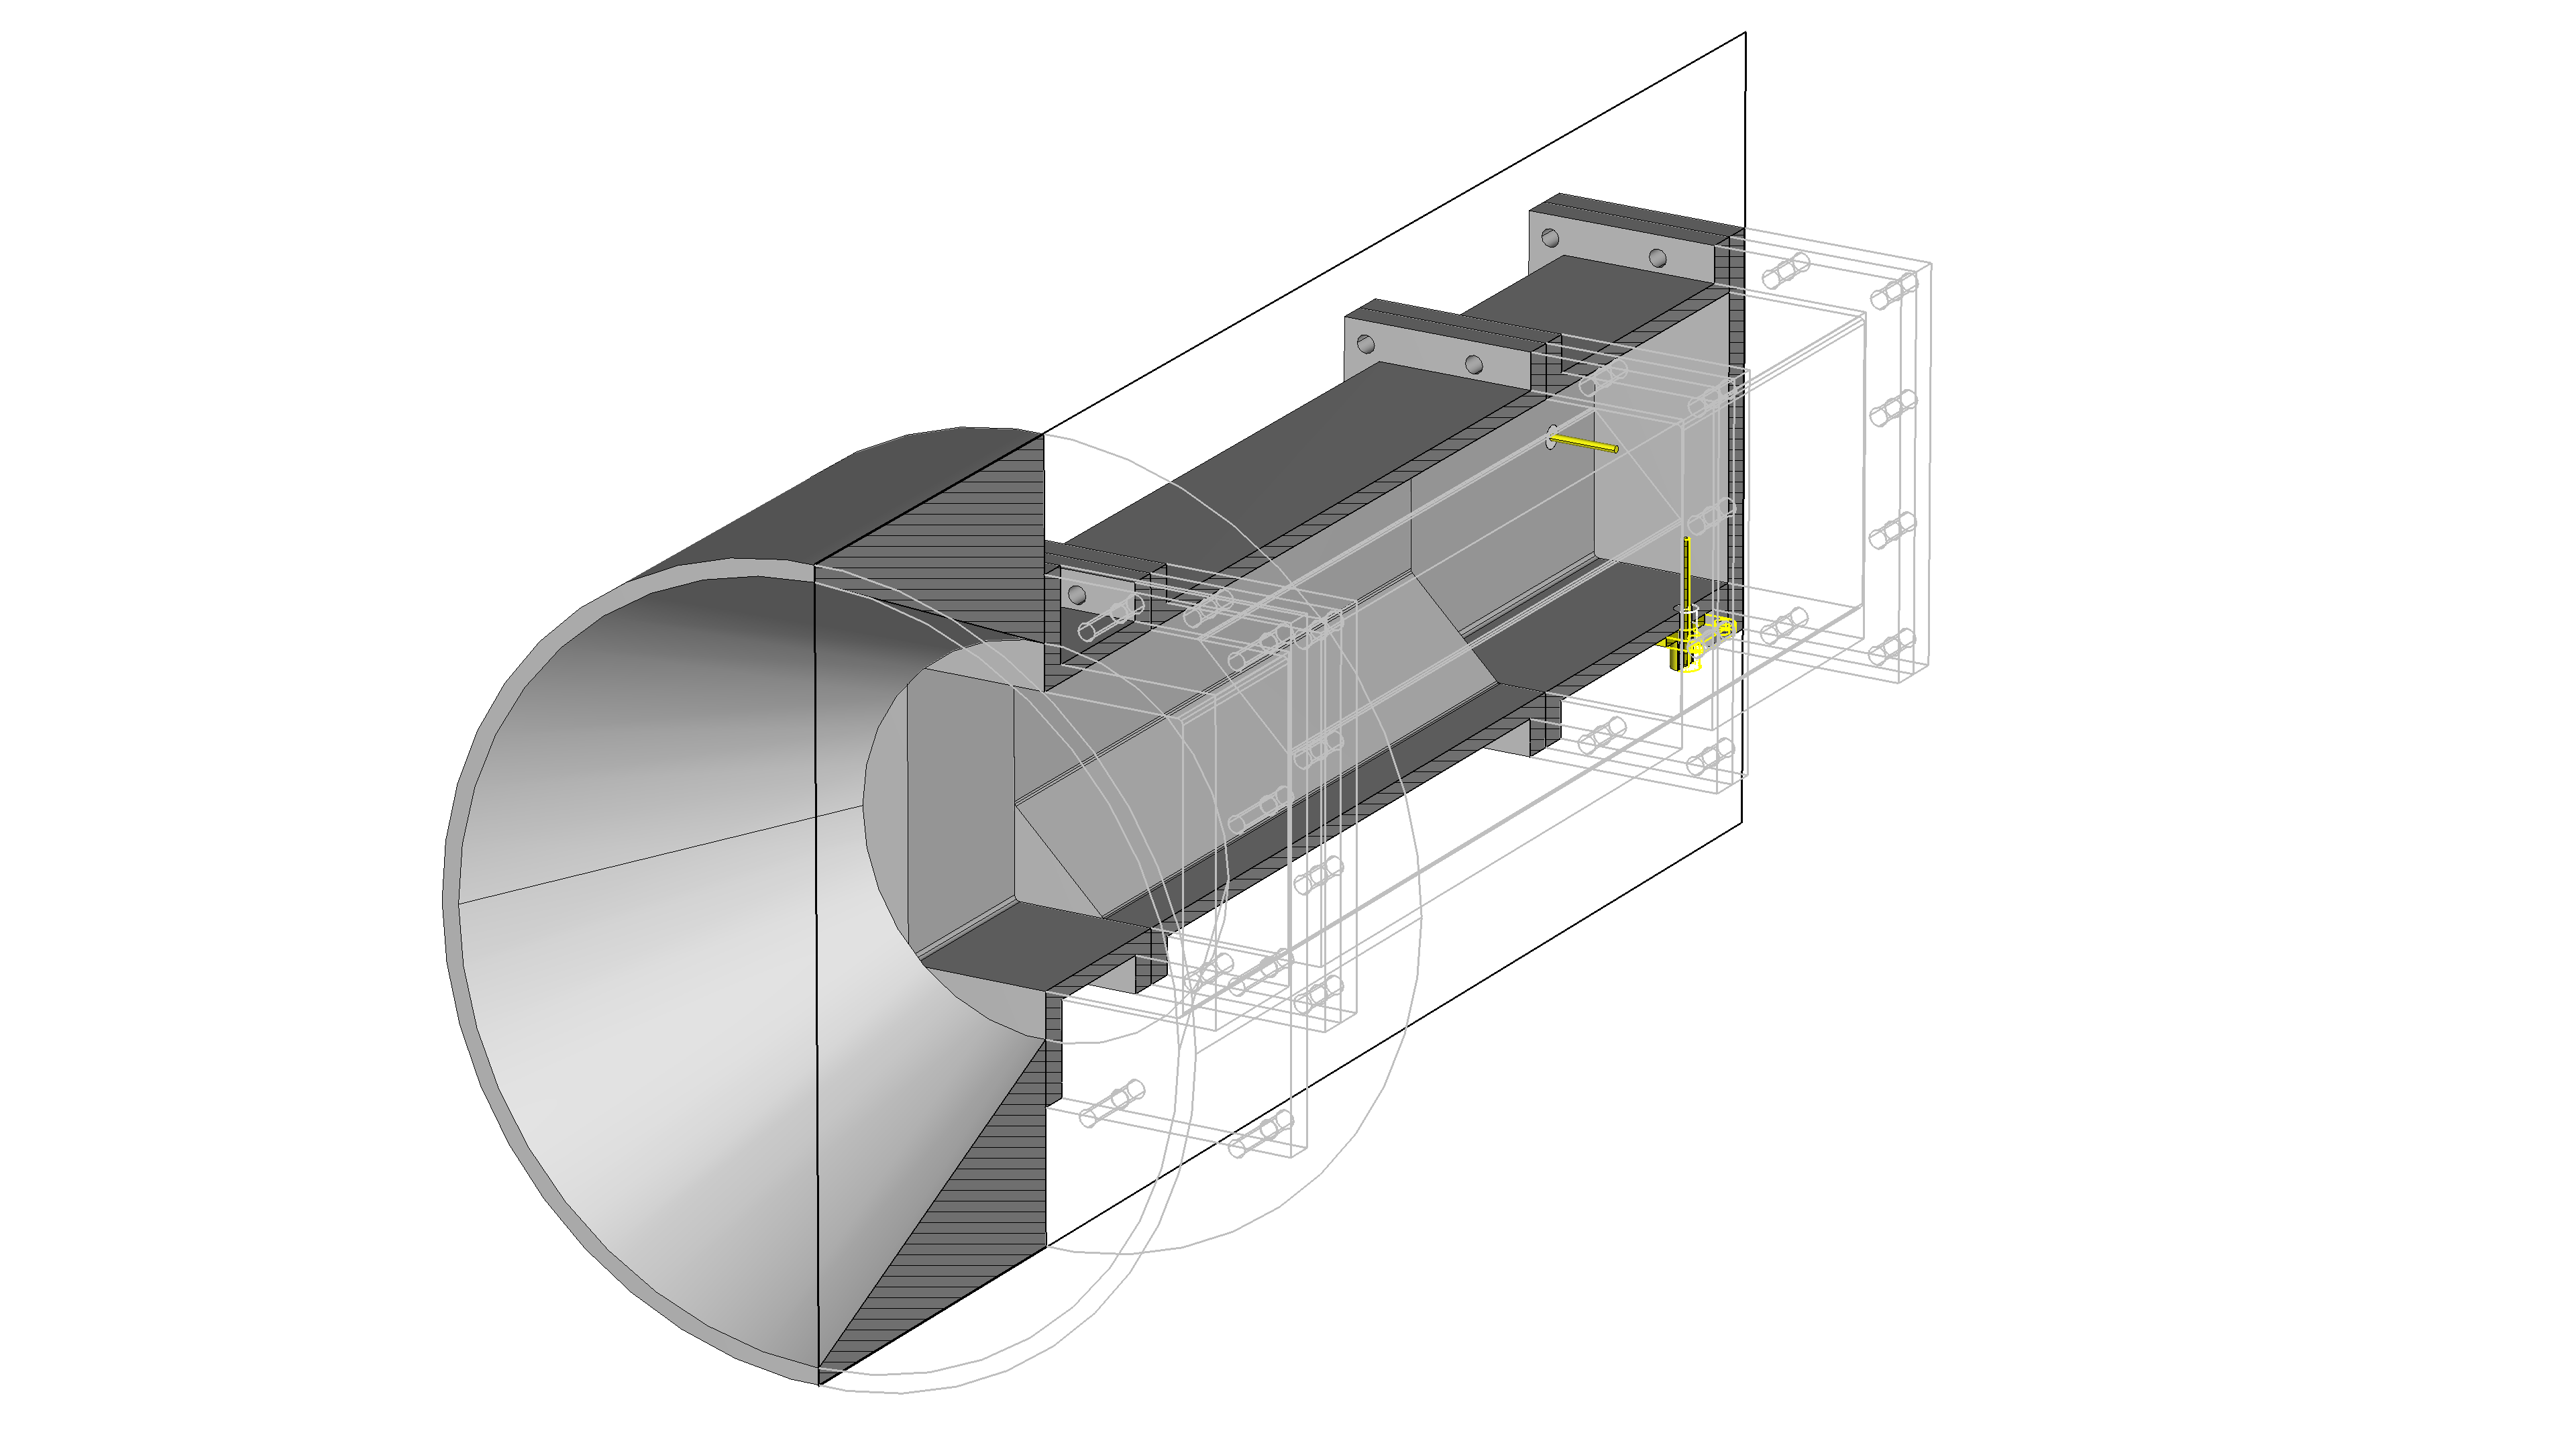
\includegraphics[width=\linewidth]{src/final_perspective.png}
\caption{\label{fig:final-perspective}Exploded view of the Design for Manufacturing (DFM)-compliant antenna model, highlighting its modular construction. The modules are numbered from front to back: 1)~conical horn antenna, 2)~square waveguide section, 3)~hexagonal waveguide polarizer, 4)~simplified dual-feed structure, and 5)~back-short wall.}
\end{figure}

To overcome this challenge, we propose a dual-feed structure that utilizes a wire-grating polarizer to isolate the two ports, inspired by the concept presented in~\cite{karki-et-al:dual-polarized-probe-for-planar-near-field-measurement}. As depicted in Fig.~\ref{fig:dual-feed-conceptual}, the two orthogonal probes (Port~1 and Port~2) are longitudinally displaced. A wire grating, oriented parallel to the electric field of the mode excited by Port~2, is placed between them. This grating is designed to be effectively transparent to the vertically polarized wave from Port~1 while acting as a reflecting surface, or a virtual back-short, for the horizontally polarized wave from Port~2. This arrangement allows both probes to maintain their optimal back-short distances---$d_1$ for Port~1 relative to the physical back-short, and $d_2$ for Port~2 relative to the grating---while achieving significant physical separation.

The design and optimization of this structure involve several critical considerations. The primary new parameter is the distance, $d_g$, between Port~1 and the wire grating. While the grating is largely transparent to Port~1, it is not perfect and introduces reflections. The back-short and the grating form a resonant cavity for Port~1, leading to sharp degradation in the reflection coefficient, $S_{11}$, at specific frequencies. The resonant frequency of this cavity is inversely proportional to the grating distance $d_g$. Analysis reveals that while a grating distance of $d_g \approx \lambda_g/4$ provides a local minimum for the reflection coefficient ($S_{11}$), port isolation ($S_{21}$) improves with increasing $d_g$. A grating distance of $d_g \approx 3\lambda_g/4$ was found to provide a superior trade-off between reflection and isolation, consistent with findings reported in~\cite{karki-et-al:dual-polarized-probe-for-planar-near-field-measurement}. The final optimization also includes the grating's geometry, specifically the wire radius, $r$, and the gap between wires, $g$, which control its reflectivity and, consequently, the performance of Port~2 and the overall port isolation.

\begin{figure}[!b]
\centering
\includegraphics[width=\linewidth]{src/final_sparameters.eps}
\caption{\label{fig:final-sparameters}Comparison of measured and simulated S-parameters for the fabricated prototype with the simplified feed.}
\end{figure}

The multi-variable optimization of all key parameters, $\{d_1, l_1, d_g, d_2, l_2, r, g\}$, was performed using the Nelder-Mead Simplex method, implemented in Python via the SciPy library~\cite{virtanen-et-al:scipy}. The optimization process was automated by a custom Python script, which systematically adjusted the design variables and evaluated their impact on the antenna's performance. This script interfaces directly with CST Studio Suite by leveraging its dedicated Python libraries~\cite{cst:python-libraries-documentation}, enabling external control of the simulation environment. For each optimization step, the script updates the CST model parameters, executes geometry checks and adjustments, and launches a new electromagnetic simulation. The resulting S-parameters are retrieved and analysed to compute an objective function that simultaneously minimizes the reflection coefficients ($S_{11}$ and $S_{22}$) and maximizes port-to-port isolation (minimizing $S_{21}$) over the specified frequency range. This iterative process continues until convergence is achieved, with the script ensuring that the best parameter set is saved upon completion or exit.

The final design demonstrates excellent performance (see Fig.~\ref{fig:dual-feed-sparameters}), with return loss for both ports remaining above $\qty{10}{dB}$ and port-to-port isolation ($S_{21}$ and $S_{12}$) better than $\qty{40}{dB}$ across the operational band. A minor ripple in the simulated S-parameters near $\qty{4.94}{GHz}$ is attributed to a weak cavity resonance between the back-short and the grating. This effect, a consequence of the grating's finite transparency, is expected to be negligible in practice due to conductor losses. However, it underscores the critical role of grating design in the antenna's overall performance.

\begin{figure}[!b]
\centering
\includegraphics[width=\linewidth]{src/final_boresight_radiation.eps}
\caption{\label{fig:final-boresight-radiation}Comparison of measured and simulated boresight gain and axial ratio. Due to the structure's symmetry, the performance is identical for both LHCP (Port 1) and RHCP (Port 2).}
\end{figure}

\subsection{Integration and Design Simplification}

While the wire-grating feed demonstrated excellent simulated isolation as a standalone component, full-wave analysis of the integrated antenna system revealed complex coupling effects between the feed, polarizer, and horn that were not present in component-level simulations. To ensure robust performance and streamline manufacturability, a simplified feed topology was adopted for the final prototype. This implementation places the two orthogonal coaxial probes in the same transverse plane, accepting a moderate trade-off in port isolation for improved system-level performance and predictability.


% ========== Section IV: Experimental Validation ==========
\section{Experimental Validation}
\label{sec:experimental-validation}

To validate the final antenna design, a prototype incorporating the simplified dual-feed structure was fabricated and measured. This approach prioritized system integration robustness and manufacturability. For fabrication, the antenna was modularized into five flanged sections (antenna, waveguide, polarizer, dual-feed, and back-short), as shown in Fig.~\ref{fig:final-perspective}.

The measured and simulated S-parameters are compared in Fig.~\ref{fig:final-sparameters}. The return loss for both ports ($S_{11}$, $S_{22}$) remains above $\qty{10}{dB}$ across the operating band, indicating a good impedance match. The port isolation ($S_{21}$, $S_{12}$) also stays above $\qty{10}{dB}$. The slight difference in return loss between Port 1 and Port 2 is due to reflections from the subsequent polarizer sections, which have different cross-sectional geometries for each port. Conversely, the port coupling is perfectly symmetrical because the primary contribution comes from the immediate coupling between neighbouring probes, which is identical for both ports.

Radiation properties were measured in an anechoic chamber. Fig.~\ref{fig:final-boresight-radiation} presents the boresight realized gain and AR. The measured gain ranges from $\qty{12}{dBi}$ to $\qty{15}{dBi}$, and the AR remains below $\qty{4}{dB}$ for both ports, confirming successful dual-CP operation. Radiation patterns%
    \footnote{The symmetry of the waveguide components ensures that the radiation pattern in the elevation plane from Port~1 is identical to the radiation pattern in the azimuth plane from Port~2, and vice versa. Furthermore, the azimuthal and elevation planes exhibit similar performance; hence, the patterns are presented only for Port~1.}
presented in Fig.~\ref{fig:final-radiation} show excellent agreement between measurement and simulation, validating the overall design.

Notably, the measured gain is slightly higher and the axial ratio lower than predicted by simulation. This discrepancy may be attributed to a combination of factors. Possible causes include measurement uncertainties (such as calibration errors, chamber reflections, or misalignment), manufacturing tolerances that resulted in smoother surfaces or more optimal dimensions than modelled, and material properties differing from those assumed in simulation (e.g., lower actual losses). Additionally, minor assembly imperfections or connector effects could have influenced the results. Overall, the combined effect of these factors likely accounts for the observed differences.

\begin{figure}[!t]
\centering
\subfloat[]{\includegraphics[width=.45\textwidth]{src/final_radiation_pattern_azimuth.eps}}
\\
\subfloat[]{\includegraphics[width=.45\textwidth]{src/final_radiation_pattern_elevation.eps}}
\caption{\label{fig:final-radiation}(a) Measured and simulated co-polarization radiation pattern for Port 1 at $\qty{5.2}{GHz}$ in the azimuthal plane ($\varphi=\ang{0}$). (b) Measured and simulated co-polarization radiation pattern for Port 1 at $\qty{5.2}{GHz}$ in the elevation plane ($\varphi=\ang{90}$).}
\end{figure}


% ========== Section V: Conclusion ==========
\section{Conclusion}
\label{sec:conclusion}

This letter presented the design and validation of a compact dual circularly polarized waveguide antenna operating in the $\frequencyrange$ frequency band. We introduced a novel antenna architecture that integrates a hexagonal waveguide polarizer, a conical horn, and a robust, manufacturable feeding structure. Experimental measurements of the fabricated prototype confirmed its strong performance, demonstrating a gain of $\qtyrange{12}{15}{dBi}$, an axial ratio below $\qty{4}{dB}$, and port isolation exceeding $\qty{10}{dB}$ across the operational band.

Additionally, our work proposed a high-isolation feeding structure concept, which achieved over $\qty{40}{dB}$ of simulated isolation. This finding provides a valuable path forward for future dual-polarized antenna designs, particularly for applications where high isolation is critical and manufacturing constraints are less restrictive. The proposed antenna and its associated design concepts offer a promising solution for satellite communications, radar, and other wireless systems requiring high-performance dual circular polarization.


% ========== Data Availability Statement ==========
\section*{Data Availability Statement}
\label{sec:data-availability-statement}

The data and code that support the findings of this study are openly available in the IEEE DataPort repository at \url{https://dx.doi.org/10.21227/hpze-c192}. The archived material includes:
\begin{itemize}
    \item Optimization script: The Python script used for the dynamic optimization of the dual-feed geometry, which externally controls CST Studio Suite.
    \item Plotting scripts: The MATLAB~\cite{matlab} scripts used for plots and calculations presented in the manuscript.
    \item Measurement and simulation data: The raw S-parameter, radiation pattern, and parametric sweep data used for the plots and calculations presented in the manuscript.
\end{itemize}


% ========== Acknowledgments ==========
\section*{Acknowledgments}
\label{sec:acknowledgments}

The authors would like to express their sincere gratitude to Universal Microwave Technology, Inc. for their crucial support in this research. We thank them for the fabrication of the antenna prototype and for performing the S-parameter measurements. Without their expertise and resources, the experimental validation of this work would not have been possible. We are also thankful for their timely and professional communication during the final stages of the project.
% \clearpage


% ========== Bibliography ==========
% \clearpage
\begin{thebibliography}{99}
    
    \bibitem{jia-et-al:dual-circularly-polarized-antennas-with-low-cross-polarization-for-gnss-r-applications}
    Y.~Jia, G.~Dassano, and P.~Savi, ``Dual circularly polarized antennas with low cross-polarization for GNSS-R applications,'' in \emph{12th European Conference on Antennas and Propagation (EuCAP 2018)}, London, UK, 2018, pp. 1--5, doi: 10.1049/cp.2018.0904.

    \bibitem{zang-et-al:single-layer-dual-circularly-polarized-antenna-elements-for-automotive-radar-at-77-ghz}
    Z.~Zang, A.~U. Zaman, J.~Yang, C.~Bencivenni, and K.~Konstantinidis, ``Single layer dual circularly polarized antenna elements for automotive radar at 77 GHz,'' in \emph{2021 15th European Conference on Antennas and Propagation (EuCAP)}, Dusseldorf, Germany, 2021, pp. 1--4, doi: 10.23919/EuCAP51087.2021.9411028.

    \bibitem{shuliak-et-al:modern-microwave-polarizers-and-their-electromagnetic-characteristics}
    V.~Shuliak, S.~Piltyay, A.~Bulashenko, I.~Zabegalov, and O.~Bulashenko, ``Modern microwave polarizers and their electromagnetic characteristics,'' in \emph{2021 IEEE 3rd Ukraine Conference on Electrical and Computer Engineering (UKRCON)}, Lviv, Ukraine, 2021, pp. 21--26, doi: 10.1109/UKRCON53503.2021.9575879.

    \bibitem{arora-et-al:dielectric-polarizer-based-potter-horn-antenna-for-deep-space-on-board-ttc-uplink-applications}
    S.~Arora, P.~V. Sitaraman, B.~S. Reddy, C.~Sriharsha, and V.~S. Kumar, ``Dielectric polarizer based potter horn antenna for deep space on-board TTC uplink applications,'' in \emph{2017 IEEE Applied Electromagnetics Conference (AEMC)}, Aurangabad, India, 2017, pp. 1--2, doi: 10.1109/AEMC.2017.8325632.

    \bibitem{melendro-jimenez-et-al:a-novel-logarithmic-spiral-shaped-3d-printed-dielectirc-polarizer-for-dual-circularly-polarized-conical-beam-radiation-patterns-in-the-ka-band}
    J.~Melendro-Jiménez, P.~Sanchez-Olivares, A.~Tamayo-Domínguez, J.~L. Masa-Campos, and J.-M. Fernández-González, ``A novel logarithmic-spiral-shaped 3-D-printed dielectric polarizer for dual-circularly polarized conical-beam radiation patterns in the Ka-band,'' \emph{IEEE Transactions on Antennas and Propagation}, vol.~72, no.~8, pp. 6219--6228, Aug. 2024, doi: 10.1109/TAP.2024.3415423.

    \bibitem{ruiz-cruz-et-al:compact-reconfigurable-waveguide-circular-polarizer}
    J.~A. Ruiz-Cruz, M.~M. Fahmi, M.~Daneshmand, and R.~R. Mansour, ``Compact reconfigurable waveguide circular polarizer,'' in \emph{2011 IEEE MTT-S International Microwave Symposium}, Baltimore, MD, USA, 2011, pp. 1--4.

    \bibitem{wang-et-al:novel-square-rectangle-waveguide-septum-polarizer}
    X.~Wang, X.~Huang, and X.~Jin, ``Novel square/rectangle waveguide septum polarizer,'' in \emph{2016 IEEE International Conference on Ubiquitous Wireless Broadband (ICUWB)}, Nanjing, China, 2016, pp. 1--4.

    \bibitem{song-et-al:design-of-wideband-quad-ridge-waveguide-polarizer}
    H.~Song, L.~Jia, J.~Tan, Y.~Zhang, and S.~Liu, ``Design of wideband quad-ridge waveguide polarizer,'' in \emph{2023 4th China International SAR Symposium (CISS)}, Xian, China, 2023, pp. 1--6.

    \bibitem{virone-et-al:optimum-iris-set-concept-for-waveguide-polarizers}
    G.~Virone, R.~Tascone, O.~A. Peverini, and R.~Orta, ``Optimum-iris-set concept for waveguide polarizers,'' \emph{IEEE Microwave and Wireless Components Letters}, vol.~17, no.~3, pp. 202--204, Mar. 2007.

    \bibitem{piltyay-et-al:new-tunable-iris-post-square-waveguide-polarizers-for-satelliste-information-systems}
    S.~Piltyay, A.~Bulashenko, H.~Kushnir, and O.~Bulashenko, ``New tunable iris-post square waveguide polarizers for satellite information systems,'' in \emph{2020 IEEE 2nd International Conference on Advanced Trends in Information Theory (ATIT)}, Kyiv, Ukraine, 2020, pp. 342--348.

    \bibitem{yu-et-al:a-wideband-circularly-polarized-horn-antenna-with-a-tapered-elliptical-waveguide-polarizer}
    H.-Y. Yu, J.~Yu, X.~Liu, Y.~Yao, and X.~Chen, ``A wideband circularly polarized horn antenna with a tapered elliptical waveguide polarizer,'' \emph{IEEE Transactions on Antennas and Propagation}, vol.~67, no.~6, pp. 3695--3703, Jun. 2019.

    \bibitem{rud-shpachenko:polarizers-on-sections-of-square-waveguides-with-inner-corner-ridges}
    L.~A. Rud and K.~S. Shpachenko, ``Polarizers on sections of square waveguides with inner corner ridges,'' in \emph{2011 VIII International Conference on Antenna Theory and Techniques}, Kyiv, Ukraine, 2011, pp. 338--340.

    \bibitem{bhardwaj-volakis:hexagonal-waveguides-new-class-of-waveguides-for-mmwave-circularly-polarized-horns}
    S.~Bhardwaj and J.~Volakis, ``Hexagonal waveguides: New class of waveguides for mm-wave circulaly polarized horns,'' in \emph{2018 International Applied Computational Electromagnetics Society Symposium (ACES)}, Denver, CO, USA, 2018, pp. 1--2.

    \bibitem{bhardwaj-volakis:hexagonal-waveguide-based-circularly-polarized-horn-antennas-for-submmwave-terahertz-band}
    S.~Bhardwaj and J.~L. Volakis, ``Hexagonal waveguide based circularly polarized horn antennas for sub-mm-wave/terahertz band,'' \emph{IEEE Transactions on Antennas and Propagation}, vol.~66, no.~7, pp. 3366--3374, Jul. 2018.

    \bibitem{bhardwaj-volakis:circularly-polarized-horn-antennas-for-terahertz-communications-using-differential-mode-dispersion-in-hexagonal-waveguides}
    S.~Bhardwaj and J.~L. Volakis, ``Circularly polarized horn antennas for terahertz communications using differential-mode dispersion in hexagonal waveguides,'' in \emph{2017 IEEE International Symposium on Antennas and Propagation \& USNC/URSI National Radio Science Meeting}, San Diego, CA, USA, 2017, pp. 2571--2572, doi: 10.1109/APUSNCURSINRSM.2017.8073328.

    \bibitem{garcia-marin-masa-campos:bowtie-shaped-radiating-element-for-single-and-dual-circular-polarization}
    E.~Garcia-Marin, J.~L. Masa-Campos, P.~Sanchez-Olivares, and J.~A. Ruiz-Cruz, ``Bow-tie-shaped radiating element for single and dual circular polarization,'' \emph{IEEE Transactions on Antennas and Propagation}, vol.~68, no.~2, pp. 754--764, Feb. 2020.

    \bibitem{armin-et-al:modification-of-a-2g2hz-sband-rectangular-patch-microstrip-antenna-using-truncated-corner-method-for-satellite-applications}
    F.~Armin, A.~Noer, Kamirul, and S.~Prasetya, ``Modification of 2.2 GHz S-Band rectangular patch microstrip antenna using truncated corner method for satellite applications,'' in \emph{2020 3rd International Seminar on Research of Information Technology and Intelligent Systems (ISRITI)}, Yogyakarta, Indonesia, 2020, pp. 284--288, doi: 10.1109/ISRITI51436.2020.9315475.

    \bibitem{cst}
    Dassault Syst{\`e}mes, \emph{CST Studio Suite, Release 2024.5, 2024}. [Online]. Available: \url{https://www.3ds.com/products-services/simulia/products/cst-studio-suite}.

    \bibitem{spinner:waveguide-specifications}
    H.-U. Nickel, ``Cross reference for hollow metallic waveguides,'' SPINNER GmbH, Tech. Rep. TD-00036, Jul. 2024. [Online]. Available: \url{https://www.spinner-group.com/images/download/technical_documents/SPINNER_TD00036.pdf}. [Accessed: Dec. 29, 2024].

    \bibitem{antenna-magus}
    Dassault Syst{\`e}mes, \emph{Antenna Magus, Release 2024.05, 2024}. [Online]. Available: \url{https://www.3ds.com/products-services/simulia/products/antenna-magus}.

    \bibitem{aboserwal-et-al:conical-horn-gain-and-amplitude-patterns}
    N.~A.~Aboserwal, C.~A.~Balanis, and C.~R.~Birtcher, ``Conical Horn: Gain and Amplitude Patterns,'' \emph{IEEE Transactions on Antennas and Propagation}, vol.~61, no.~7, pp.~3427--3433, Jul. 2013, doi: 10.1109/TAP.2013.2256453.

    \bibitem{fabregas-et-al:coaxial-to-rectangular-waveguide-transitions}
    I.~Fabregas, K.~Shamsaifar, and J.~M. Rebollar, ``Coaxial to rectangular waveguide transitions,'' in \emph{IEEE Antennas and Propagation Society International Symposium 1992 Digest}, Chicago, IL, USA, 1992, pp. 2122--2125~vol.4, doi: 10.1109/APS.1992.221447.

    \bibitem{karki-et-al:dual-polarized-probe-for-planar-near-field-measurement}
    S.~K. Karki, J.~Ala-Laurinaho, and V.~Viikari, ``Dual-polarized probe for planar near-field measurement,'' \emph{IEEE Antennas and Wireless Propagation Letters}, vol.~22, no.~3, pp. 576--580, Mar. 2023, doi: 10.1109/LAWP.2022.3218731.

    \bibitem{cst:python-libraries-documentation}
    Dassault Syst\`emes Deutschland GmbH, \emph{CST Python Libraries}. [Online]. Available: \url{https://space.mit.edu/RADIO/CST_online/Python/main.html}. [Accessed: 29 December 2024].

    \bibitem{virtanen-et-al:scipy}
    P.~Virtanen \emph{et al.}, ``SciPy 1.0: Fundamental Algorithms for Scientific Computing in Python,'' \emph{Nature Methods}, vol.~17, pp. 261--272, 2020, doi: 10.1038/s41592-019-0686-2. [Online]. Available: \url{https://rdcu.be/b08Wh}

    \bibitem{matlab}
    The MathWorks, Inc. (2025). \emph{MATLAB version: 25.1.0.2943329 (R2025a)}. [Online]. Available: \url{https://www.mathworks.com}
\end{thebibliography}


\end{document}
